\documentclass{article}
\usepackage{hyperref}
\usepackage{amsmath} % or simply amstext
\newcommand{\angstrom}{\textup{\AA}}

\title{Physical Chemistry Problems and Why We Care}
\usepackage{Sweave}
\begin{document}
\Sconcordance{concordance:Chemistry1.tex:Chemistry1.Rnw:%
1 6 1 1 0 54 1 1 2 1 0 2 1 5 0 1 1 6 0 1 2 22 1 1 2 1 0 1 1 6 0 1 2 89 %
1 1 2 1 0 3 1 1 2 1 1 3 0 2 2 7 0 2 1 4 0 1 2 18 1 1 2 1 0 2 1 6 0 2 1 %
4 0 1 2 17 1}

\maketitle

\section{Introduction}

There are several concepts in \emph{physical chemistry} that turn out to have wide applications and we are going to explore some of them here. 

First, we should acknowledge that the early history is filled with people who had the luxury to explore rather esoteric topics, while we might be learning these as a matter of our own `development' and with a sense of what for!  I'll try to make an argument that this stuff really does matter, but for now, let's start the problem set!

Second, we also need to understand that these assignments have been developed as hurtles that have almost nothing to do with the end-goal of being a health-care professional. Instead, it's better to reflect that being able to think about problem solving is actually the real goal here and we need to learn to problem solve in a systematic way.


\section{Problem \#2}

\subsection{Background}
Neutron radiation is a kind of ionizing radiation which consists of free neutrons. A result of nuclear fission or nuclear fusion, it consists of the release of free neutrons from atoms, and these free neutrons react with nuclei of other atoms to form new isotopes, which, in turn, may produce radiation.

Cold, thermal and hot neutron radiation is most commonly used for scattering and diffraction experiments in order to assess the properties and the structure of materials in crystallography, condensed matter physics, biology, solid state chemistry, materials science, geology, mineralogy and related sciences. Neutron radiation is also used in select facilities to treat cancerous tumors due to its highly penetrating and damaging nature to cellular structure. Neutrons can also be used for imaging of industrial parts termed neutron radiography when using film, neutron radioscopy when taking a digital image, such as through image plates, and neutron tomography for three-dimensional images. Neutron imaging is commonly used in the nuclear industry, the space and aerospace industry, as well as the high reliability explosives industry.

The imaging is a function of the particles wavelength, $\lambda$, where higher freqencies resolve higher resolution. It's rare that one would ever have to calculate this from scratch, but the value of the exercise is ??? 

\subsection{de Brogie Wavelenth}

In 1923, Louis de Broglie, a French physicist, proposed a hypothesis to explain the theory of the atomic structure. By using a series of substitution de Broglie hypothesizes particles to hold properties of waves. Within a few years, de Broglie's hypothesis was tested by scientists shooting electrons and rays of lights through slits. What scientists discovered was the electron stream acted the same was as light proving de Broglie correct.

Thus, for this problem, we will determine the wavelength of a particle (nuetron), which also has a mass -- one of the strangest scientific theories!

In this problem we are trying to determine (calculate) the `de Brogie' wavelenth. So, let's first determine the units of a wavelength, so we have a clue where we are heading!  In general, wavelength is measured as length per time, in SI units, we often see this as m/s, but for atomic particle scales, the units are often \angstrom/second, where an Angstrom (\angstrom) is $1 \cdot  10^{-10}$ meters, i.e very short disances! Note: an \angstrom~ is not an SI unit, which is terribly lame. But let's let that go for now, I think $1\cdot 10^{-9}$ is the SI units, which is a nanometer.  Whatever!

We are given the a number that includes temperature, as measured in Kelvin. Okay, that seems to be a weird parameter to be given! But let's back up. We are told that a particle accelartor generate nuetrons at 2500K, where K is degrees Kelvin, i.e. a temperature. By knowing temperature, we are supposed to figure out a wavelength, weird!!!

We are given the following equation to determine velocity of the nuetron

\begin{equation}
\mu_{rms} = \sqrt{(3k_BT/m)}
\end{equation}

where $\mu_{rms}$ is room-mean-speed (m/s), $k_B$ is Boltzmann's Constant ($1.38e^{-23}$ J/K) and T is temperature (degrees K) and m is the mass of the particle (kg). This equation is the root-mean square of speed (velocity) of particles -- it's a kind of an average speed, see \url{http://www.studyphysics.ca/2007/20/ap_thermodynamics/42a_ap_kinetic_theory_gases.pdf} for a decent explanation. For now, we'll use $\mu_{rms}$ as arithmetic mean of the squares of a set of numbers). The RMS is also known as the quadratic mean and is a particular case of the generalized mean with exponent.

Thus, the $\mu_{rms}$ is
\begin{Schunk}
\begin{Sinput}
> k_B = 1.38e-23
> T = 2500
> m = 1.6750e-24; m
\end{Sinput}
\begin{Soutput}
[1] 1.675e-24
\end{Soutput}
\begin{Sinput}
> mu = sqrt(3*k_B*T/m); mu
\end{Sinput}
\begin{Soutput}
[1] 248.578
\end{Soutput}
\end{Schunk}

Thus, we have now calculated the speed as 248.58. However, I am not sure this is right. Did you get this as a intermediate answer with your prof? I need to figure out the units too!

Next, what do we do with the velocity?  

Using this site: \url{http://chem.libretexts.org/Core/Physical_and_Theoretical_Chemistry/Quantum_Mechanics/02._Fundamental_Concepts_of_Quantum_Mechanics/De_Broglie_Wavelength}, we might be able to evaluate the question with some sense that we understand what in the world is happening:

\begin{equation}
\lambda = hp = h m \nu
\end{equation}

\noindent where h is planck's constant, p is the particle momentum and m is the particle's mass and $\mu$ is the particles' velocity. 

Based on this equation, we have velocity, $\mu$, and we know the mass of the nuetron, which is 0. Thankfully, h, or Planck's Constant is a known quanity, altough we derive it in problem \#4!

\begin{Schunk}
\begin{Sinput}
> h = 6.626e-34
> lambda = h * m * mu; lambda
\end{Sinput}
\begin{Soutput}
[1] 2.758856e-55
\end{Soutput}
\end{Schunk}

At this point, I am doing something wrong, because it's hard to belive that this wavelength is so small, 0. I suspect I didn't calculate the velocity correctly, seems way too slow!

\section{On Planck's Constant}

\url{https://en.wikipedia.org/wiki/Planck_constant}



$\lambda/\angstrom$ is in the units of wavelenth per meter or meter/second/meter thus we are left with a time unit! Neat. I am not sure why they can tell us that!  The symbolism is totally weird, because the author has the \angstrom is a demonintor, but actually it's just refering to the units. 

$V_s/V$ is the stopping voltage, but the demominator is confusing, and is only refering to the units, which are in volts!

Finally, the hint is anything but a real hint -- basically driving more questions that it answers. 

The equation given is 

\begin{equation}
KE = EV_s
\end{equation}

\noindent where KE is kenetic energy (units?) and E is the charge of an electron (volts) and $V_s$ is stopping voltage.

We might be able to use the photo-electric equation,

\begin{equation}
E = h\nu
\end{equation}

\begin{Schunk}
\begin{Sinput}
> one=c(2536, 2830, 3039, 3302, 3663, 4358)
> two=c(2.6, 2.11, 1.81, 1.47, 1.1, .57)
> coef(lm(one~two))
\end{Sinput}
\begin{Soutput}
(Intercept)         two 
  4713.1565   -885.1904 
\end{Soutput}
\begin{Sinput}
> plot(one,two)
\end{Sinput}
\end{Schunk}
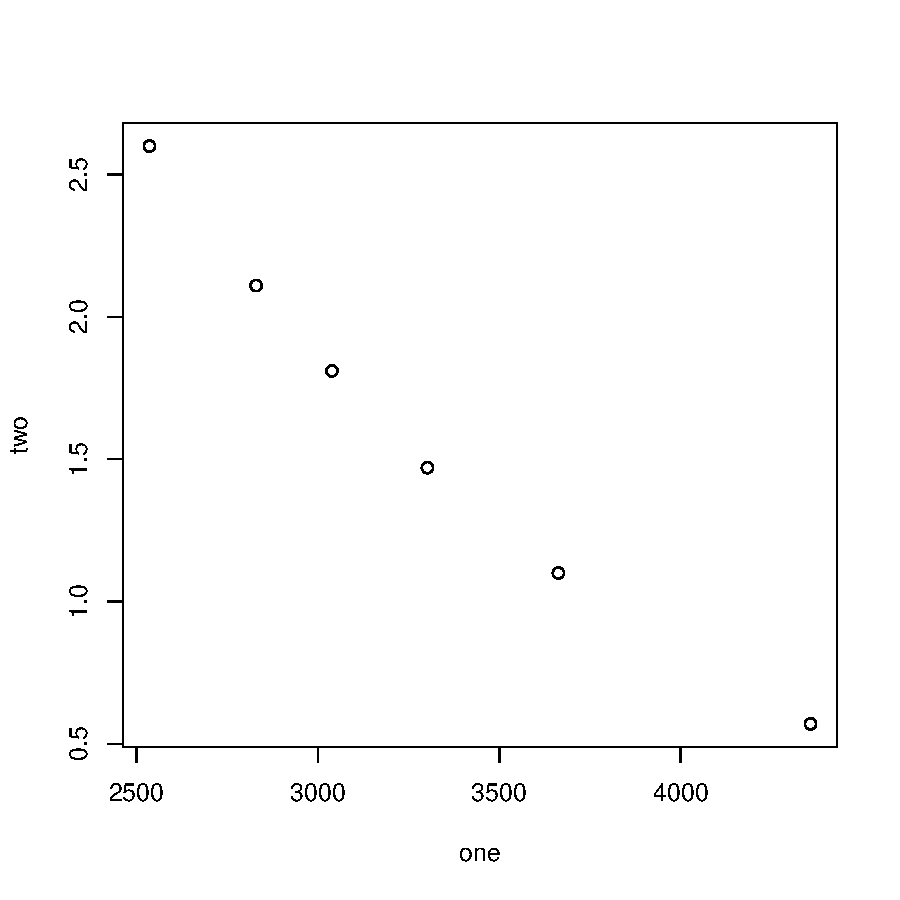
\includegraphics{Chemistry1-003}

OR?

\begin{Schunk}
\begin{Sinput}
> plot(two,one)
> coef(lm(two~one))
\end{Sinput}
\begin{Soutput}
 (Intercept)          one 
 5.217508994 -0.001097174 
\end{Soutput}
\end{Schunk}
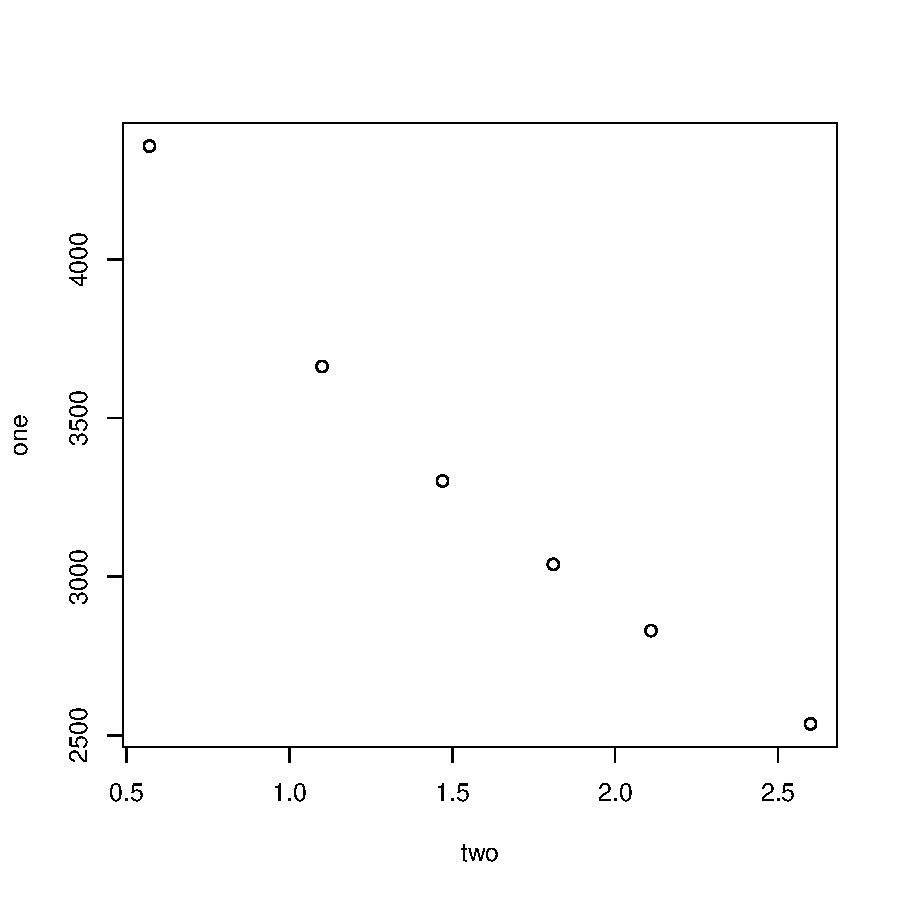
\includegraphics{Chemistry1-004}

The intercept might be E?  I didn't have time to sort this out last night and without a textbook, I am a bit lost as to what formulas we need. More later today -- i.e. Wed.

\end{document}
